	\section{Learning to adapt to opponents}
\label{sec:part3}

In the previous chapter we created an algorithm to develop the default strategy for the APC. \\

In this chapter we will answer problem statement 3.
As we did not have time to implement the adaptive part into the APC, we instead choose to focus on a more theoretically chapter.


\vspace{4mm}
\begin{statementBox2}{Problem statement 3}
How can we further develop the APC's strategy to be able to adapt to the playing style of the opponent?
\end{statementBox2}
\vspace{4mm} 


In poker there is no strategy that is better than any other strategy. Every strategy has weaknesses and therefore the optimal strategy is the one that takes advantage of the weaknesses of the strategies of the opponents. In order to take advantage of the opponents strategy, one must first understand their strategy. In poker understanding the opponents is one of the most important key elements of the game. Once a player gains insight in the opponents strategy, it is important to adapt the playing strategy accordingly.


Since poker is a game of deception the opponents' may change their strategy during the game. In this case the player needs detect this and adapt the strategy once again. 

\subsection{Design}
This chapter is focused on the theoretical aspect an adaptive part to the APC rather than the implementation and testing. The reason is, that we did not have enough time to implement it and furthermore the ANN from chapter \ref{sec:part2} did not end up being as functional as expected. Therefore it would not be possible to tell if the solution would not work, due to the original ANN or due to the improvements created in this chapter. 

Instead of implementing the improvements, we simply suggest how we could have implemented them.\\

There are two commonly used approaches to develop a strategy that adapts to the strategy of the opponents.

The traditional approach is the use of statistics to gain information about the opponent. Such an approach uses probabilities based on the opponents' actions to determine the strength of the opponents' hands. These probabilities may include, but are not limited to, the percentage of hands the opponents' folds during each game state, the percentage of times the opponents' bluffs on the river, and the strength of the hand the opponents' has when calling an aggressive player. This is useful against an opponent who uses the same strategy throughout the whole game and has deterministic actions.

The other approach is using player modelling, see section \ref{sec:pm} and artificial neural networks (ANN), see section \ref{sec:nn}. This approach has gained increasing popularity through the recent years. In this approach the ANN is responsible of learning the strategy of the opponent. This approach is also good for learning the strategy of an opponent who performs non-deterministic actions. It can also adapt in case the opponent changes strategy.\\

We choose to use the second approach and create a player model and an ANN. We find it more interesting to use player modelling and ANN's as this approach seems to have a lot of potential within the field of artificial intelligence in poker compared to the statistically approach.

Aaron Davidson is a master of science from the University of Alberta. In his thesis about opponent modelling in poker \cite{opp-mod}, he uses ANN's in combination with player modelling in order to develop the poker computer Poki. An ANN was designed to predict the action of an opponent. The ANN uses a total of 17 player specific inputs. Using this design, Poki was able to win against most online poker players and computers but was far from world class.

G. Nicolai and R. Hilderman also made use of ANN's and player modelling in their thesis \cite{poker-agents}. They use a single ANN to determine the action of their computer agent. The model each player using overall aggressiveness and recent aggressiveness and give it as an input to the ANN. Although their computer agent was no way as advanced as Poki, it still showed potential.

Using ANN's in combination with player modelling looks like reasonable approach. In the rest of this chapter, we will discuss this approach and suggest a potential way of implementing it. We will start by introducing the concept of player modelling. We then design a player model suitable for the APC and finally design the ANN.

\subsubsection{Player modelling}
\label{sec:pm}
Player modelling is a loosely defined concept and may vary from one context to another. The concept of player modelling is to make a computational model of a player. This model includes game related attributes, such as play style and preferences, as well as non-game related attributes, such as cultural background, gender, and personality. All decisions of the player are ultimately made on the basis of these attributes. 

Player modelling is used to describe or predict the opponents' decisions, reasoning, and reactions. In the field of artificial intelligences the human player is the most used model for developing computer players. Understanding the reason behind every choice of an opponent will not only bring a better understanding of the opponent but also a better understanding of the game and its dynamics.

Since the player model can easily become extremely extensive one has to determine which attributes are relevant.

\subsubsection{Design of the player model}
It is crucial that one figures out which attributes are relevant to the specific player model. When trying to model a player there is almost no limit to what could be included. Attributes such as state of mind, energy, and distractions affect the decision of every human player.  

Below we have listed the attributes that we find most relevant for a player model in poker.

\begin{description}
\item[Aggressiveness] How often does the opponent tend to bet or raise.
\item[Tightness] How strictly does the opponents actions reflect the strength of the opponents hand. For instance, a tight opponent will play aggressive when having a strong hand and defensive or fold when having a weak hand. A loose opponent may bluff (play aggressive while having a weak hand) and slow play (play defensive while having a strong hand) a lot.
\item[Riskiness] How easy is it to push the opponent to fold. Risky opponents tend to fold less often while under pressure from a player and are therefore harder to bluff against.
\item[Body language] Most human players unconsciously show emotions through their body language. The professional poker players can often tell a lot about an opponents hole cards solely by looking at the opponents body language.
\item[Time of decision making] The time an opponent uses for each decision can show the confidence of the opponents choice. A fast decision indicates an easy decision. However, the time spent on making a decision can be misleading as distractions can occur.
\end{description}

Since our APC is targeted towards computer players as well as human players, it makes no sense to use attributes such as body language and the time of decision making to model the opponents. Those attributes only affect human players. Instead we will model the opponents using the attributes aggressiveness, tightness, and riskiness.

Aggressiveness can be found by simply looking at the actions of the opponent. 

Tightness is a bit more complicated as we need to know the hole cards of the opponent. Therefore, we can only track the tightness of rounds where the opponent makes it to the showdown.

Riskiness is also easy to measure. Riskiness shows how likely the opponent is to call while under pressure from APC. We can determine the riskiness of the player by tracking the number of times the opponent folds as compared to the number of times the opponent calls or raises.

The APC needs to be able to recognise if a player changes strategy during the game. To accomplish this we split each attribute into the two attributes: overall and recent. Overall, covers every round throughout the game. Recent, only covers the last ten rounds.

The reason we choose ten rounds, in our definition of recent, is because a player might get lucky and get several strong hole cards in a row. This may cause the player to play more aggressive than usual even though the player still uses the same strategy - resulting in a miss read by the player model. We found that ten games is enough to avoid miss-reads and also allows to track actual changes in the players strategy.

Aggressiveness is also split into one additional attribute called current aggressiveness, which is the players aggressiveness in previous game states of the current round.

We end up using the following attributes for our player model:
\begin{itemize}
\item Overall aggressiveness
\item Recent aggressiveness
\item Current aggressiveness
\item Overall tightness
\item Recent tightness
\item Overall riskiness
\item Recent riskiness
\end{itemize}

In the rest of this section we will describe one way we could have implemented the player model. Note that the player model has not been implemented but this is only a description of how we would have done it.

The aggressiveness of a round $n$ can be found as:

\[Agg,n = \frac{A_{bet},n + A_{raise},n}{A_{total},n}\]

$A_{agg},n$ is the opponents' number of bets $A_{bet},n$ and raises $A_{raise},n$ in round $n$ and  $A_{total},n$ is the opponents' total number of actions in round $n$. 

Overall aggressiveness can be found as the average aggressiveness of all rounds, recent aggressiveness is found as the average aggressiveness of the last ten rounds and finally the current aggressiveness is found as the average aggressiveness of the previous game states of the current round.\\

The tightness of the opponent can is found by backtracking the actions of the opponent after the round is finished. This is of course only possible for rounds that makes it to the showdown, since we otherwise do not know the hole cards of the opponents.

In order to determine if a player either bluffs or slow plays, we would have to establish some boundaries based on the hand strength. 

We took a sample of 100 defensive actions and 100 aggressive actions, and inserted the data in figure \ref{fig:dist-act}. The boundary for bluffing (red line) shows that the players tends to play defensive below this line. Likewise, the boundary for slow play (blue line) shows that the players tends to play aggressive above this line.

\begin{figure}[H]
  \center
    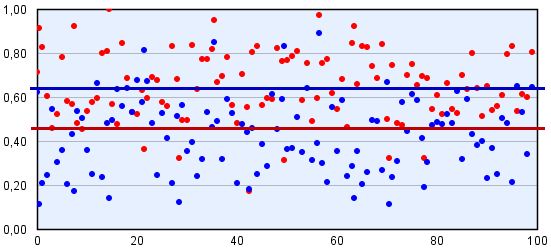
\includegraphics[scale=0.775]{images/modeling/action-dist.png}
  \caption{Distribution of actions in regards to the hand strength. Red dots indicates aggressive actions and blue dots defensive actions. The red line indicates the boundary for slow play and the blue line the boundary for bluffing. \label{fig:dist-act}}
\end{figure}

We define slow playing as playing defensive with a hand strength of more than 0,63.

We define bluffing as playing aggressive with a hand strength of less than 0,46.

We can then find the tightness of a round $n$ using the formula:

\[Ti,n = 1 - \frac{A_{bluff},n + A_{slow},n}{A_{total},n}\]

Here $A_{bluff},n$ is the number of times the player has bluffed in round $n$, $A_{slow},n$ is the number of times the player has slow played in round $n$ and $A_{total},n$ is the total number of actions in round $n$.

We can then find the overall- and recent tightness the same way as with the aggressiveness. Although we can only track the past ten rounds where the player made it to showdown.\\

Finally we can find the riskiness of a round $n$ as the number of times the player calls or raises in regards to the number of times it costs the player to continue:

\[Ri,n = \frac{A_{call},n + A_{raise},n}{A_{call},n + A_{raise},n + A_{fold},n}\]

Here we have the number of times the player calls $A_{call},n$, raises $A_{raise},n$ and folds $A_{fold},n$, all in round $n$.

\subsection{Combining the ANN and player model}
The ANN for the adaptive strategy would be based on the ANN design from section \ref{sec:design2}, see figure \ref{fig:nn2}. 


We choose to use the approach by G. Nicolai and R. Hilderman and construct a single ANN that takes the attributes of the players as inputs. The target is to learn the ANN what to do, based on the inputs about the game and attributes of the opponents.

The inputs for the ANN can be seen in table \ref{tab:ann-design}. The attributes of the players are the attributes found in the previous section. In case there is less than nine opponents all attributes of a non-existing player is set to zero. Since the input function finds the net input as the sum of all the weighted inputs all inputs that are zero will not affect the ANN.

\begin{table}[H]
\center
\begin{tabular}{ | l | l | }
\hline
input & feature \\
\hline
1 & hand strength of APC\\
2 & number of opponents\\
3 & chips of the APC\\
4 & cost of the APC\\
5 & pot\\
6 to 12 & attributes of opponent 1\\
13 to 19 & attributes of opponent 2\\
20 to 26 & attributes of opponent 3\\
27 to 33 & attributes of opponent 4\\
34 to 40 & attributes of opponent 5\\
41 to 47 & attributes of opponent 6\\
48 to 54 & attributes of opponent 7\\
55 to 61 & attributes of opponent 8\\
62 to 68 & attributes of opponent 9\\
\hline
\end{tabular}
\caption{Inputs for the ANN design \label{tab:ann-design}}
\end{table} 

\subsection{Discussion}
We discuss how we could have improved the strategy of the APC to also take the opponent's play style into account. Since we have no tests it is close to impossible to say if our solution would work or not.

We choose to use player modelling to model the opponents using seven attributes. The three main attributes we choose are aggressiveness, tightness, and riskiness. All these attributes are used to say something about the play style of the player. Other attributes more specific to the game state might also be worth considering such as: chips of the player, position of the player, the amount of chips the player has already committed in this round.
Most of the inputs used for Poki are all related to the game state rather than the play style. 

We believe that it is a good idea to put all the attributes of the player model as inputs to the ANN. This way we can always try to remove some of the inputs or add new ones in order to measure if the TNE of the ANN gets lower. This way it would be fairly easy to test which attributes that has an impact on the result. 

Because of the huge amount of inputs the ANN would probably have to redesigned so it have more hidden neurons.\\

All together this approach seems very adaptable and easy to modify in order to incrementally test the ANN with attributes of different player models.


\subsection{Conclusion}
In this chapter we discuss and suggest a solution to problem statement 3.

\vspace{4mm}
\begin{statementBox2}{Problem statement 3}
How can we further develop the APC's strategy to be able to adapt to the playing style of the opponent?
\end{statementBox2}
\vspace{4mm} 

For our approach we use player modelling to find relevant attributes to define an opponent. These attributes will then be given as inputs to an ANN which then determines the action of the APC. 

To make it possible for the APC to detect changes in the strategy of an opponent, we find two attributes: an overall attribute and a recent attribute. A change in strategy will affect the recent attribute and cause the APC to detect the change.

We ended up having a total of seven attributes.\\

We suggest the following way of finding the attributes:

The aggressiveness of a round can be found as the number of times the opponent bets or raise divided by the total number of actions of the opponent for that round.

The aggressiveness of a round can be found as the number of times the opponent bluffs or slow plays divided by the total number of actions of the opponent for that round.

The riskiness of a round can be found as the number of times the opponent calls or raises divided by the total number of times the opponent has to pay in order to continue.\\

By designing a new ANN that takes the attributes for each opponent as additionally inputs, we believe that the ANN with its 68 inputs have the information it needs to adapt to opponents.
